\documentclass[11pt]{article}
\usepackage{worksheet_style}

% ---- Toggle: uncomment for filled version ----
%\worksheetfilledtrue
\begin{document}
\worksheetheader{6}{Functions of Several Variables}

\begin{background}
This is where Calculus III truly begins. Until now we've worked with vectors and curves---extensions of familiar geometry. Starting today, we study functions $f(x,y)$ and $f(x,y,z)$ that take multiple inputs and return a single output. Temperature at a point in a room, pressure in the atmosphere, cost as a function of two inputs---these are all multivariate functions. We need new tools to visualize them (level curves, cross-sections) and new techniques to analyze them (partial derivatives, gradients, multiple integrals). Everything from here to the end of the course builds on this foundation.
\end{background}

%=============================================================
\wsection{Functions of Two Variables}

\begin{defbox}{Function of Two Variables}
A \textbf{function of two variables} $f:D\subseteq\R^2\to\R$ assigns to every point $(x,y)$ in its domain a single real number $f(x,y)$. Whereas a single-variable function $y=f(x)$ draws a curve in the plane, a two-variable function draws a \textbf{surface} in 3D: for each input $(x,y)$ you plot the point $(x,y,f(x,y))$, and the set of all such points is the \textbf{graph} $z=f(x,y)$. Think of the $(x,y)$-plane as the ``floor'' and the surface as a landscape whose height above that floor is determined by $f$.

-- The graph $z = f(x,y)$ is a \wbi{surface in $\R^3$}{3.5cm}
\end{defbox}

\begin{center}
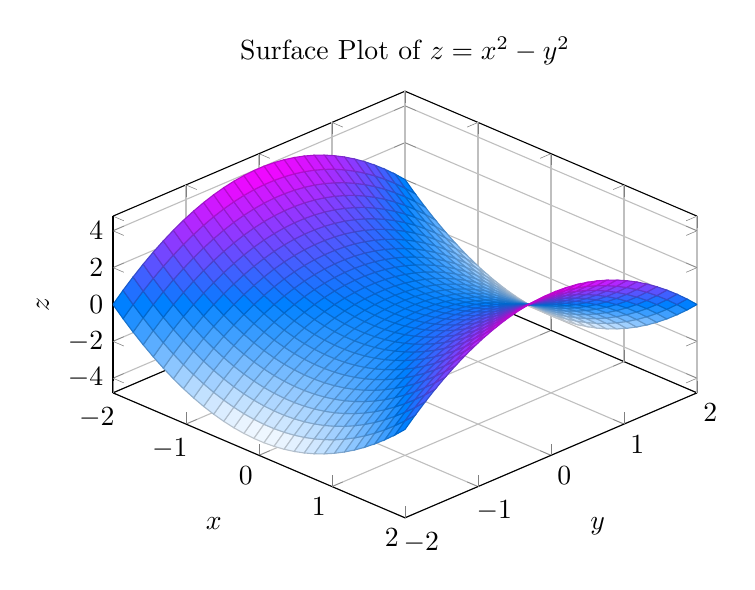
\begin{tikzpicture}
\begin{axis}[
    view={45}{45},
    xlabel={$x$}, ylabel={$y$}, zlabel={$z$},
    colormap/cool,
    grid=major,
    domain=-2:2,
    y domain=-2:2,
    samples=30,
    z buffer=sort,
    title={Surface Plot of $z = x^2 - y^2$},
    width=9cm, height=7cm
]
\addplot3[surf] {x^2 - y^2};
\end{axis}
\end{tikzpicture}\\
{\small Graph of $z=f(x,y)$ as a 3D surface. Each point $(x,y)$ in the plane is lifted to height $f(x,y)$; here $z=x^2-y^2$ is the classic saddle.}
\end{center}

\begin{example}[Real-World Multivariable Functions]
Write each as $f(\text{inputs})$:
\begin{enumerate}[label=(\alph*), nosep]
  \item Ohm's Law: $V = \wbm{IR}$ \; ($V$ depends on current $I$ and resistance $R$)
  \item Kinetic energy: $KE = \wbm{\frac{1}{2}mv^2}$ \; (depends on mass $m$ and velocity $v$)
  \item Ideal gas law: $P = \wbm{\frac{nRT}{V}}$ \; (at fixed $n,R$: depends on $T$ and $V$)
\end{enumerate}
\end{example}

%=============================================================
\wsection{Domains and Ranges}

\begin{formulabox}{Domain Restrictions to Watch For}
\begin{itemize}[nosep, leftmargin=*]
  \item \textbf{Denominators} -- cannot equal $0$
  \item \textbf{Square roots} -- argument $\geq 0$
  \item \textbf{Logarithms} -- argument $> 0$
  \item \textbf{Inverse trig} -- $|\text{argument}| \leq 1$ (for arcsin, arccos)
\end{itemize}
\end{formulabox}

\begin{example}[Finding Domains]
Find the domain of each function:
\begin{enumerate}[label=(\alph*)]
  \item $\ds f(x,y) = \frac{1}{x+y}$

  \wbbox{
  \textbf{1. Restriction:} $x+y \neq 0$

  \textbf{2. Result:} $\dom(f) = \{(x,y) : y \neq -x\}$ -- all of $\R^2$ except the line $y=-x$

  Range: $(-\infty, 0) \cup (0, \infty)$
  }{2.5cm}

  \item $\ds g(x,y) = \frac{\ln(x-y)}{\sqrt{x^2+y^2-4}}$

  \wbbox{
  \textbf{1. Restrictions:} $x - y > 0$ (for $\ln$) AND $x^2+y^2-4 > 0$ (for $\sqrt{}$ in denominator)

  \textbf{2. Result:} $\dom(g) = \{(x,y) : x > y \text{ and } x^2+y^2 > 4\}$

  -- Region below the line $y = x$ and outside the circle of radius 2
  }{3cm}
\end{enumerate}
\end{example}

%=============================================================
\wsection{Level Curves}

\begin{defbox}{Level Curves}
A \textbf{level curve} (or \textbf{contour}) of $f(x,y)$ at height $k$ is the set of all points in the $(x,y)$-plane where $f$ takes the value $k$ — equivalently, the horizontal slice of the graph at height $z=k$, projected down onto the floor. Drawing many of these for different values of $k$ produces a \textbf{topographic map} of the surface: regions where curves are packed close together correspond to \emph{steep} parts of the surface, while widely-spaced curves correspond to gentle slopes.
\[\{(x,y) : f(x,y) = k\}\]
\end{defbox}

\begin{center}
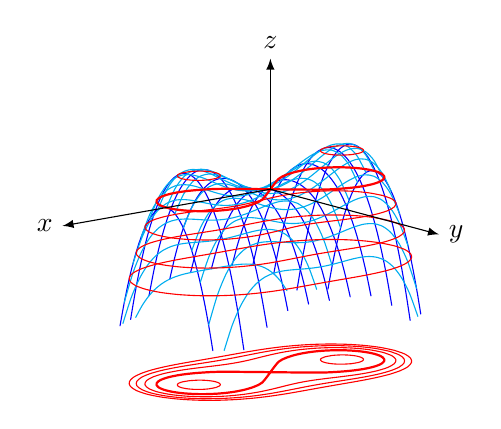
\begin{tikzpicture}[scale=1.7,line cap=round,line join=round,
   x={(-0.7766cm,-0.1369cm)},y={(0.6300cm,-0.1688cm)},z={(0cm,0.9761cm)}]
\def\xmin{1}
\def\ymin{0.7}
\pgfmathsetmacro\xstep{\xmin-0.2}
\pgfmathsetmacro\ystep{\ymin-0.1}
\def\h{-1.4}
\foreach\i in{-\xmin,-\xstep,...,\xmin}
{
  \pgfmathsetmacro\xdom{min(\ymin,sqrt(-0.5-\i*\i+0.5*sqrt(5+8*\i*\i)))}
  \draw[blue] plot[domain=-\xdom:\xdom,samples=25,smooth]
    (\i,\x,{-(\i*\i+\x*\x)*(\i*\i+\x*\x)+(\i*\i-\x*\x)});
}
\foreach\i in{-\ymin,-\ystep,...,\ymin}
{
  \pgfmathsetmacro\xdom{min(\xmin,sqrt(0.5-\i*\i+0.5*sqrt(5-8*\i*\i)))}
  \draw[cyan] plot[domain=-\xdom:\xdom,samples=25,smooth]
    (\x,\i,{-(\x*\x+\i*\i)*(\x*\x+\i*\i)+(\x*\x-\i*\i)});
}
\foreach\a in {0,180} \foreach\z in {0,\h}
{
  \draw[thick,red] plot[domain=-45+\a: 45+\a,samples=25,smooth]
    ({sqrt(cos(2*\x))*cos(\x)},{sqrt(cos(2*\x))*sin(\x)},\z);
}
\def\z{0.2}
\pgfmathsetmacro\xdom{0.5*acos(2*sqrt(\z))-0.005}
\foreach\zz in {\z,\h} \foreach\a in {0,180} \foreach\s in {-1,1}
{
  \draw[red] plot[domain=\a-\xdom:\a+\xdom,samples=25,smooth]
    ({sqrt(0.5*cos(2*\x)+0.5*\s*sqrt(cos(2*\x)*cos(2*\x)-4*\z))*cos(\x)},
     {sqrt(0.5*cos(2*\x)+0.5*\s*sqrt(cos(2*\x)*cos(2*\x)-4*\z))*sin(\x)},\zz);
}
\foreach\z in {-0.2,-0.4,-0.6} \foreach\zz in {\z,\h}
{
  \draw[red] plot[domain=-180:180,samples=51,smooth]
   ({sqrt(0.5*cos(2*\x)+0.5*sqrt(cos(2*\x)*cos(2*\x)-4*\z))*cos(\x)},
    {sqrt(0.5*cos(2*\x)+0.5*sqrt(cos(2*\x)*cos(2*\x)-4*\z))*sin(\x)},\zz);
}
\draw[-latex] (0,0,0) -- (2,0,0) node[left]  {$x$};
\draw[-latex] (0,0,0) -- (0,2,0) node[right] {$y$};
\draw[-latex] (0,0,0) -- (0,0,1) node[above] {$z$};
\end{tikzpicture}\\
{\small A 3D surface with its level curves projected straight down onto the $xy$-plane. The infinity-shaped level curve is a Bernoulli lemniscate. Together, the surface and its contour projection give complementary views of the same function.}
\end{center}

\begin{formulabox}{Plotting Level Curves}
\begin{enumerate}[nosep]
  \item Choose several values of $k$ in the range of $f$
  \item For each $k$, set $f(x,y) = k$ and simplify
  \item Identify and sketch each resulting 2D curve
  \item Label each curve with its $k$-value
\end{enumerate}
\end{formulabox}

\begin{example}[Level Curves of a Paraboloid]
Sketch level curves of $f(x,y) = x^2 + y^2$ for $k = 1, 4, 9, 16$.

\wbbox{
\textbf{1. Set up:} $x^2 + y^2 = k$ -- circles of radius $\sqrt{k}$

\textbf{2. Identify curves:}
\begin{itemize}[nosep]
  \item $k=1$: circle of radius 1
  \item $k=4$: circle of radius 2
  \item $k=9$: circle of radius 3
  \item $k=16$: circle of radius 4
\end{itemize}

\textbf{3. Result:} Concentric circles -- they get closer together as $k$ increases (steeper slope at higher $z$).
}{5cm}
\end{example}

\begin{example}[Level Curves of a Saddle]
Sketch level curves of $f(x,y) = x^2 - y^2$ for $k = -4, -1, 0, 1, 4$.

\wbbox{
\textbf{1. Set up:} $x^2 - y^2 = k$

\textbf{2. Identify curves:}
\begin{itemize}[nosep]
  \item $k > 0$: hyperbolas opening along the $x$-axis
  \item $k < 0$: hyperbolas opening along the $y$-axis
  \item $k = 0$: $y = \pm x$ (two lines through origin)
\end{itemize}

\textbf{3. Result:} Topographic map of a hyperbolic paraboloid (saddle surface). Two families of hyperbolas cross at the saddle point.
}{4cm}
\end{example}

%=============================================================
\wsection{Common 3D Equations}

\begin{formulabox}{Surfaces You Should Recognize}
\begin{center}
\begin{tabular}{ll}
\toprule
\textbf{Equation} & \textbf{Surface} \\
\midrule
$x^2+y^2+z^2 = r^2$ & \wbi{Sphere}{3cm} \\
$x^2+y^2 = r^2$ & \wbi{Cylinder}{3cm} \\
$z = x^2+y^2$ & \wbi{Paraboloid}{3cm} \\
$x^2+y^2 = z^2$ & \wbi{Cone}{3cm} \\
$z = x^2-y^2$ & \wbi{Saddle (hyperbolic paraboloid)}{3cm} \\
$Ax+By+Cz = D$ & \wbi{Plane}{3cm} \\
\bottomrule
\end{tabular}
\end{center}
\end{formulabox}

%=============================================================
\wsection{Functions of Three or More Variables}

\begin{defbox}{Level Surfaces}
For $f: \R^3 \to \R$, we cannot graph $w = f(x,y,z)$ (requires 4D). Instead we use \textbf{level surfaces}:
\[\{(x,y,z) : f(x,y,z) = k\}\]
-- The 3D analog of level curves
\end{defbox}

\begin{example}[Level Surfaces of $x^2+y^2+z^2$]
Describe the level surfaces of $f(x,y,z) = x^2 + y^2 + z^2$.

\wbbox{
\textbf{1. Set up:} $x^2+y^2+z^2 = k$

\textbf{2. Identify:}
\begin{itemize}[nosep]
  \item $k > 0$: spheres of radius $\sqrt{k}$ centered at the origin
  \item $k = 0$: single point (the origin)
  \item $k < 0$: empty set
\end{itemize}

\textbf{3. Result:} $f$ measures squared distance from origin, so level surfaces are concentric spheres.
}{3.5cm}
\end{example}

%=============================================================
\begin{practice}

\prob
Find the domain of $f(x,y) = \sqrt{9 - x^2 - y^2}$.

\wans{\wbml{$x^2+y^2 \leq 9$ -- the closed disk of radius 3}}

\vspace{2cm}

\prob
Find the domain and range of $f(x,y) = e^{-(x^2+y^2)}$.

\wbbox{
Domain: all of $\R^2$ (exponent always defined).

Range: $(0, 1]$. Max $f=1$ at origin; $f \to 0$ as $\|(x,y)\| \to \infty$.
}{2.5cm}

\prob
Sketch level curves of $f(x,y) = xy$ for $k = -2, -1, 0, 1, 2$.

\wbbox{
$xy = k \implies y = k/x$: hyperbolas with asymptotes on the axes.

$k=0$: the axes themselves ($x=0$ or $y=0$).

$k>0$: curves in Q1 and Q3. \; $k<0$: curves in Q2 and Q4.
}{3cm}

\prob
Describe the level surfaces of $T(x,y,z) = 100 - x^2 - y^2 - z^2$.

\wbbox{
$T = k \implies x^2+y^2+z^2 = 100-k$. Spheres of radius $\sqrt{100-k}$ centered at origin.

Valid for $k \leq 100$. Max temperature $T=100$ at origin.
}{3cm}

\prob
The wind chill index is $W(v, T) = 35.74 + 0.6215T - 35.75v^{0.16} + 0.4275Tv^{0.16}$. Find $W$ at $T = 0^\circ$F and $v = 25$ mph. What do the level curves represent physically?

\wbbox{
$v^{0.16} = 25^{0.16} \approx 1.673$

$W = 35.74 + 0 - 35.75(1.673) + 0 = 35.74 - 59.83 \approx -24.1^\circ$F

Level curves $W = k$: combinations of wind speed and temperature that ``feel'' the same.
}{4cm}

\end{practice}

\end{document}
